
\newpage
\section{One Dimensional Minimization and Direct Search}


\begin{definition}[Unimodal Function]\label{def:unimodal_fnc}
A function \( f : [a,b] \to \R \) is called unimodal if there exists a \( \xi \in [a,b] \), so that
\( f \) is strictly decreasing in \( [a, \xi] \) and strictly increasing in \( [\xi, b] \).
\end{definition}
\bigskip

In fact \( \xi \) is the unique minimum of \( f \) in \( [a, b] \). According to the definition, 
for \( a \le x < y \le b \) we have 
\[
    f(x) > f(y) \text{ for } x, y \in [a, \xi) \text{ and } f(x) < f(y) \text{ for }  x, y \in (\xi, b]
\]
Thus
\[
    \xi \in [a, y] \text{ if } f(x) < f(y) \text{ and } \xi \in [x, b] \text{ if } f(x) \ge f(y)
\]
Let now \( [a_0, b_0] = [a, b] \) and \(a_0 \le x_0 < y_0 \le b_0 \). Furthermore
\[
    [a_{k + 1}, b_{k + 1}] = 
        \begin{cases}
            [a_k, y_k] & \text{ if } f(x_k) < f(y_k)  \\
            [x_k, b_k] & \text{ if } f(x_k) \ge f(y_k)
        \end{cases}
\]
for \( a_k \le x_k < y_k \le b_k \) respectively. It follows that \( [a_k, b_k] \supset [a_{k + 1}, b_{k + 1}] \) 
is a decreasing series of intervals.

Consider the following partioning of the interval \( [0, 1] \) where the following relations hold 
\[
     x = 1 - y \text{ and } \\ \frac{1}{y} = \frac{y}{x}
\]

Thus \( 1 - y = y^2 \) and
\[ 
     y = \frac{\sqrt{5} - 1}{2}
\]
\bigskip

\algorithm[Line Search]\label{algo:golden_section_search}\hfill
\bigskip
\inputminted{python}{golden_section.py}
\bigskip

NO2TEST

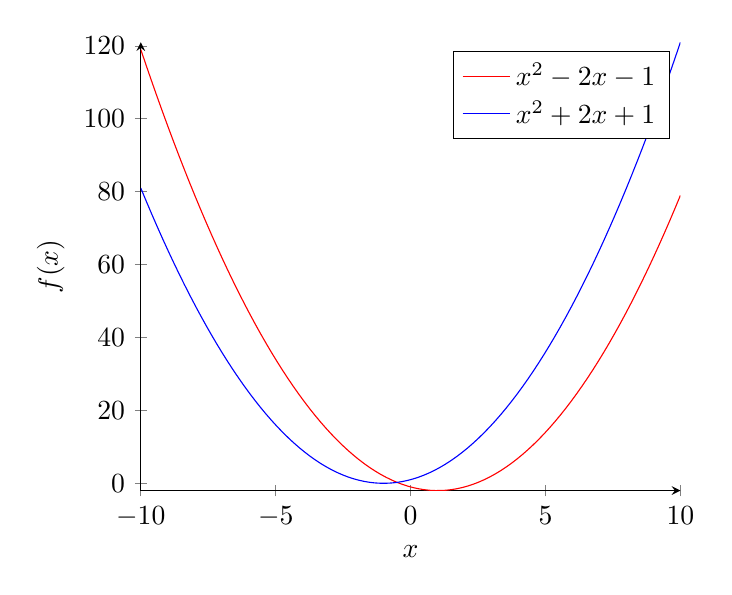
\begin{tikzpicture}
\begin{axis}[
    axis lines = left,
    xlabel = $x$,
    ylabel = {$f(x)$},
]
\addplot [
    domain=-10:10, 
    samples=100, 
    color=red,
]
{x^2 - 2*x - 1};
\addlegendentry{$x^2 - 2x - 1$}
\addplot [
    domain=-10:10, 
    samples=100, 
    color=blue,
    ]
    {x^2 + 2*x + 1};
\addlegendentry{$x^2 + 2x + 1$}
\end{axis}
\end{tikzpicture}

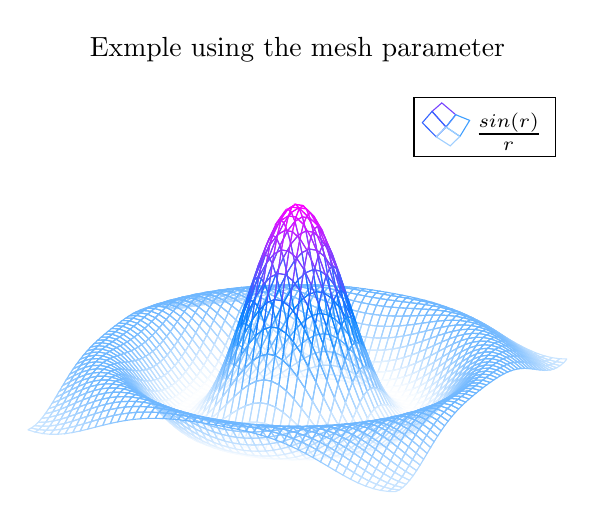
\begin{tikzpicture}
\begin{axis}[
    title=Exmple using the mesh parameter,
    hide axis,
    colormap/cool,
]
\addplot3[
    mesh,
    samples=50,
    domain=-8:8,
]
{sin(deg(sqrt(x^2+y^2)))/sqrt(x^2+y^2)};
\addlegendentry{$\frac{sin(r)}{r}$}
\end{axis}
\end{tikzpicture}